\chapter{Processi aziendali}
\label{chap:processi-metodologie}

\section{Organizzazione e collaborazione}
Lo stage si inserisce nel progetto \textit{ErpAI} di Spazio Dev, con l’obiettivo di realizzare il primo motore di previsione degli acquisti integrato nell’ERP proprietario. Il team conta un referente tecnico aziendale, due sviluppatori e il sottoscritto; lo sviluppo del modulo di previsione e delle componenti di explainable AI è assegnato a me. Le procedure sono in evoluzione perché l’azienda è giovane e in crescita, ma già orientate a documentazione condivisa, verifiche automatizzate e tracciabilità delle decisioni.

\subsection{Ambienti e strumenti di sviluppo}
L’azienda consente a ciascun sviluppatore di utilizzare il proprio sistema operativo e l’IDE preferito, nel rispetto delle convenzioni di progetto. La coerenza tra i team è garantita dalla containerizzazione: tutti i progetti sono eseguiti in Docker e, quando serve un ambiente di sviluppo replicabile, viene adottato ddev. Quest’ultimo offre configurazioni preimpostate e comandi uniformi per avviare i servizi, aggiornare le dipendenze e verificare l’applicazione in locale. Ne derivano onboarding più rapido, dipendenze allineate e test eseguiti in ambienti equivalenti a quelli usati per l’integrazione continua.

\subsection{Modello di lavoro agile}
Il framework adottato è Scrum\footnote{\url{https://it.wikipedia.org/wiki/Scrum_(informatica)}}, che articola il lavoro in iterazioni brevi con fasi di pianificazione, sviluppo, revisione e retrospettiva. I titolari di Spazio Dev esercitano il ruolo di Product Owner definendo priorità, obiettivi di Sprint e criteri di accettazione, e quello di Scrum Master coordinando le cerimonie e rimuovendo gli impedimenti. Gli sviluppatori, incluso il sottoscritto, realizzano le attività di backlog, rendicontano gli avanzamenti e presentano gli incrementi. Ogni Sprint settimanale si apre con la definizione del lavoro da eseguire per \textit{ErpAI} e si chiude con la verifica degli incrementi consegnati e la retrospettiva sui miglioramenti di processo.
\begin{figure}[H]
    \centering
    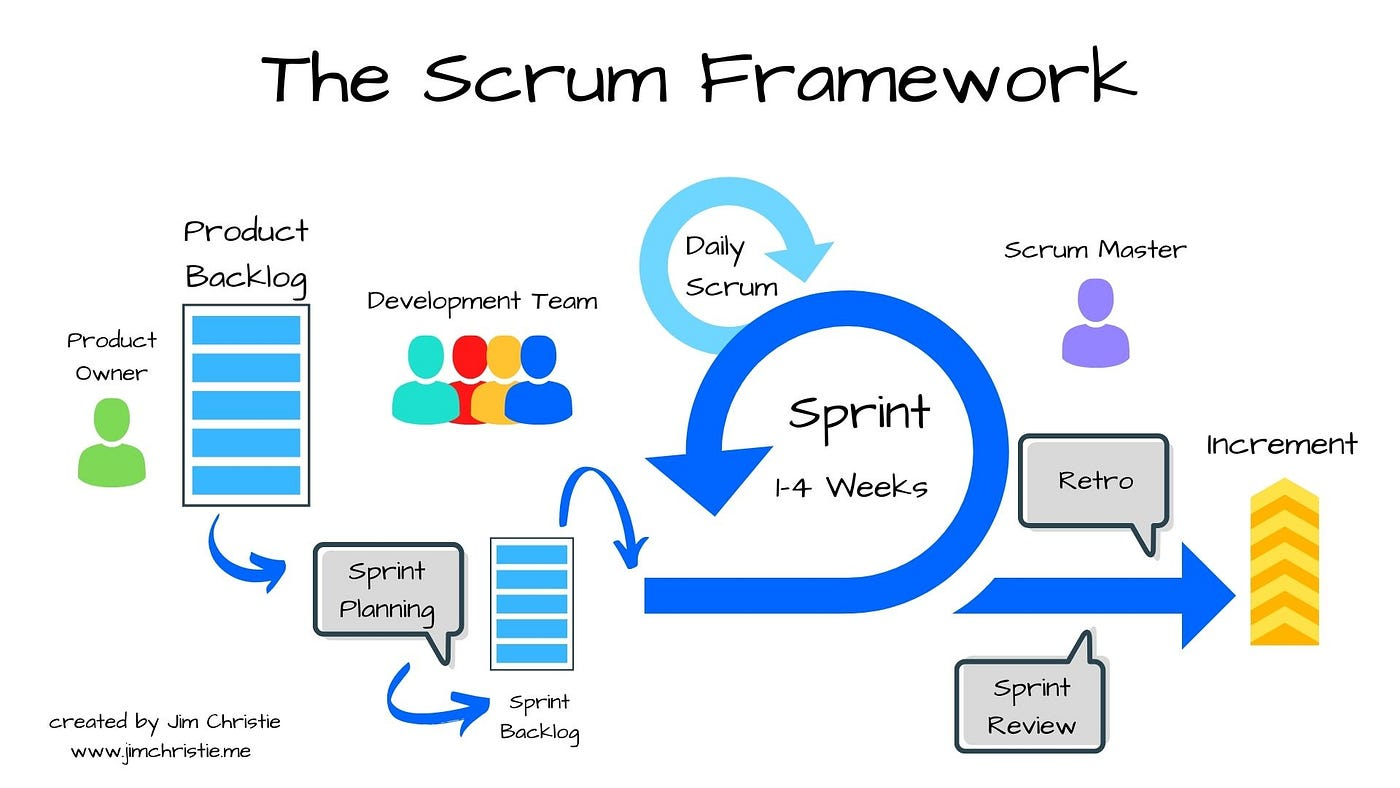
\includegraphics[alt={Schema del framework Scrum adottato}, width=0.9\linewidth]{img/framework_scrum.jpg}
    \caption{Schema semplificato del framework Scrum adottato}
    \label{fig:scrum-framework}
\end{figure}

\subsection{Comunicazione e documentazione}
La comunicazione avviene su canali Telegram dedicati a ciascun progetto, dove team e referenti si scambiano aggiornamenti quotidiani, e durante le cerimonie Scrum già descritte. Per la documentazione si utilizza la sezione \textit{Pages} di Plane, accessibile a tutti i membri del progetto, affiancata dai file nel repository (README, note operative). Per questo lavoro è presente anche una documentazione OpenAPI che descrive le REST API sviluppate.

\section{Strumenti tecnici e controllo qualità}

\subsection{Version control e branching}
Il codice è gestito con Git\footnote{\url{https://git-scm.com/}}, sistema di controllo versione distribuito, e ospitato su Gitea\footnote{\url{https://about.gitea.com/}}, piattaforma self-hosted per repository e merge request. È adottato un modello di branching ispirato a Gitflow ma ridotto alle necessità del progetto:
\begin{itemize}
    \item \textbf{main}: contiene le versioni rilasciabili e sincronizzate con l’ERP;
    \item \textbf{develop}: integra in modo continuo le attività in corso;
    \item \textbf{feature/<nome>}: per lo sviluppo di nuove funzionalità;
    \item \textbf{fix/<nome>}: per correggere errori individuati in test o review;
    \item \textbf{docs/<nome>}: per aggiornamenti alla documentazione.
\end{itemize}
Ogni branch è nominato in modo descrittivo per collegare rapidamente il lavoro all’attività tracciata.

I messaggi di commit seguono lo standard \textit{Conventional Commits}\footnote{\url{https://www.conventionalcommits.org/en/v1.0.0/}} con prefissi \texttt{feat}, \texttt{fix} e \texttt{docs}, così da facilitare la lettura della cronologia e la generazione di note di rilascio.

\begin{figure}[H]
    \centering
    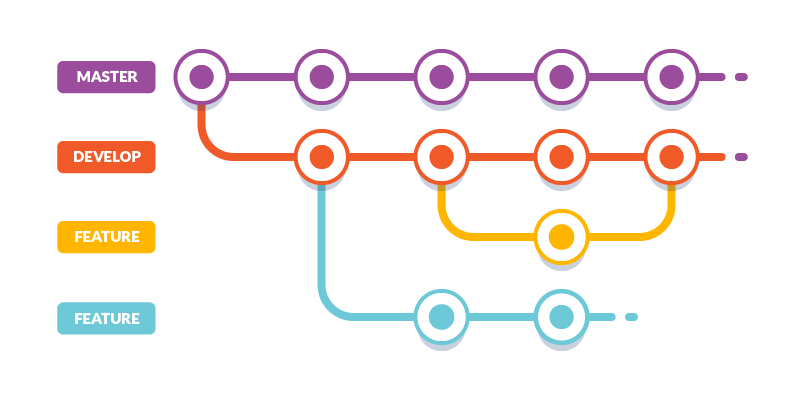
\includegraphics[alt={Schema del modello Gitflow adottato con branch main, develop e rami di feature/fix/docs}, width=0.9\linewidth]{img/gitflow_scheme.png}
    \caption{Schema del branching model adottato}
    \label{fig:gitflow-scheme}
\end{figure}

\subsection{Issue tracking}
Le attività sono tracciate su Plane\footnote{\url{https://plane.so}} con una board Kanban a quattro colonne: \textit{Backlog} raccoglie le attività proposte; \textit{Todo} contiene quelle selezionate per lo Sprint; \textit{In Progress} include il lavoro in corso; \textit{Done} raccoglie ciò che è completato.

Ogni issue include:
\begin{itemize}
\item descrizione chiara dell’attività, dell’obiettivo e dell’output atteso, sia esso una nuova feature, un bugfix o un aggiornamento documentale;
    \item livello di priorità, con valori \textit{Critical}, \textit{High}, \textit{Medium} o \textit{Low};
    \item assegnatario dell’attività, così da rendere esplicita la responsabilità e il punto di contatto;
    \item modulo del progetto a cui l’attività è collegata, utile per aggregare il lavoro per componente e verificare l’impatto.
\end{itemize}
\begin{figure}[H]
    \centering
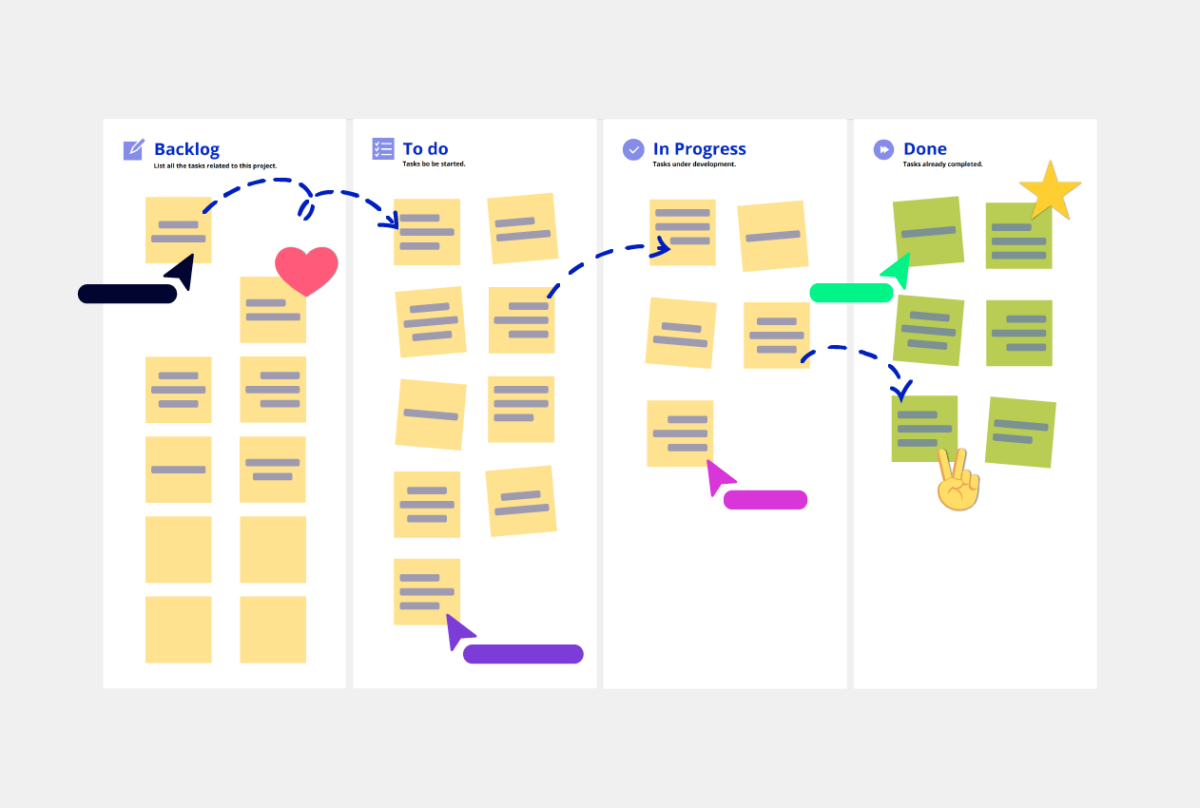
\includegraphics[alt={Esempio di board Kanban su Plane con colonne Backlog, Todo, In Progress, Done}, width=0.9\linewidth]{img/kanban_board.png}
    \caption{Schema semplificato della board Kanban su Plane}
    \label{fig:plane-board}
\end{figure}

\subsection{Testing e integrazione continua}
Per il modulo di previsione di \textit{ErpAI} è stata introdotta una pratica di integrazione continua approvata dall’azienda. Su Gitea è configurato un workflow che, a ogni push, esegue i test unitari sulle funzioni di pre-processing e sulle logiche di servizio, oltre ai test di integrazione sugli endpoint FastAPI. L’esito della pipeline è vincolante per questo modulo: solo i branch che superano i test possono essere mergiati in \texttt{main}, garantendo che il motore di previsione resti stabile prima di ogni distribuzione.



\newpage
